\textcolor{blue}{
    This section consists of three main parts. The first part is that we motivate the importance of re-optimization. Then, we characterize the fundamental limitation of traditional re-optimization. Last, we use it as motivation to introduce a new perspective of re-optimization called the sub-query perspective and a novel query processing framework called \textit{query split}.
}
    \begin{itemize}[leftmargin = 15pt]
        \item We first review the problem of cardinality estimation and explain why it is hard to accurately estimate the cardinality of complex query results (in Section \ref{S21}).
        \item Then, we review an existing query processing technique called re-optimization and discuss the underlying philosophy of re-optimization (in Section \ref{S22}).
    \textcolor{blue}{
        \item Next, we discuss shortages of the sub-plan perspective, which traditional re-optimization methods adopt (in Section \ref{S23}).
        \item Last, we propose a new perspective of re-optimization called the sub-query perspective and design a \textit{query split} framework to cooperate with this new perspective (in Section \ref{S24}).
    }
    \end{itemize}

\subsection{Intrinsic Difficulty of Cardinality Estimation} \label{S21}
    Currently, most database systems estimate cardinality as the product of three terms: the size of both relations and predicate selectivity, in which the selectivity is estimated via table statistics \cite{book1}. For example, in PostgreSQL, the selectivity of a simple predicate on base tables is estimated using gathered statistics such as histograms, most common values and their frequencies, and the number of distinct values. For conjunctive predicates, it is commonly assumed that the component predicates are independent, so the final selectivity is the product of the selectivity of each predicate \cite{JOB}. For complex join queries, independence between join predicates is often assumed, and their selectivities are multiplied together. In MySQL, the cardinality estimation strategy is very similar \cite{manual1}.\par
    There are two major reasons why it is hard to guarantee the accuracy of cardinality estimation \cite{Reopt}. The first reason is that optimizer lacks the statistics of intermediate relations. We use an example to demonstrate why this is a problem that troubles the optimizer.
    \begin{Example}
        A database contains two relations $A(a)$ and $B(a, b)$ and some statistics in the system catalog including the cardinality of two relations $n_A$ and $n_B$ and the value distribution of attributes $f_A^a$, $f_B^a$ and $f_B^b$. Given a natural join query $r=A \bowtie B$, the cardinality of $r$ is given by:\par
        $n_r=n_A \times n_B \times selec_{A,B}=n_A \times n_B \times \Sigma_{i \in dom(a)}(f_A^a(i) \times f_B^a(i))$
        where $dom(a)$ is the domain of attributes $a$.\par
        However, when we apply a filter to attribute $b$, cardinality estimation of $r$ becomes more difficult. Consider the query $r=A \bowtie \sigma_{b=x}(B)$, and denote the intermediate relation as $t=\sigma_{b=x}(B)$. So that the query can be rewritten as $r=A \bowtie t$, and the cardinality of $t$ is $n_t=n_B \times f_B^b(x)$. Since any other statistic about $t$ is unknown, the optimizer must approximate those missing statistics by some assumptions. For example, if we assume independence between attributes $a$ and $b$ in table $B$, we can get $f_t^a(i) = f_B^a(i|b=x) = f_B^a(i)$, which can then be used to estimate the selectivity of join predicate. However, those assumptions may not be actually valid, and would introduce error in estimation.\par
        Similar situation happens when the filter $\sigma_{b=x}(B)$ is replaced by a new join, e.g. $r=A \bowtie (B \bowtie C)$. Since we only have the statistics of base relations, to estimate the cardinality of the final result $n_r$, we have to assume independence across joins. Specifically, we use the selectivity of joins between base relations to approximate the selectivity of joins containing intermediate results, which also leads to estimation error.
    \end{Example}
    From the above example, we can see that the optimizer has to make assumptions to compensate for the lack of statistics, which inevitably generates estimation errors.\par
    The second reason is error propagation. Yannis and Stavros mathematically deduce that the cardinality estimation error of an N-way natural join grows exponentially with N, assuming that there is some error in estimating the distribution of join attribute in each relation \cite{paper31}. Hence, except for small queries, cardinality estimation results are often not trustworthy. Although these results are based on theoretical analysis, they are also generally valid in practice based on our empirical observations during experiments.\par

\subsection{Re-optimization} \label{S22}
    As it is hard to make cardinality estimation always accurate, Kabra and DeWitt proposed re-optimization \cite{Reopt} to circumvent this problem. Re-optimization collects statistics during run-time to monitor query execution. When the collected statistics deviate too much from prediction, the system replans the remainder of the query plan in light of this new information, which can alter join orders and physical operators of the remaining part.\par
    As shown in Figure \ref{F1}, in a re-optimization scheme, the optimizer initially provides an execution plan to be executed. Then, during the execution of the plan, we materialize the intermediate result and switch back to the optimizer with some new run-time statistics collected during materialization. With such information, the optimizer can either keep the original plan or produce another plan to be executed. This iteration can happen several times until the final result is ready.\par
    \begin{figure}
        \centering
        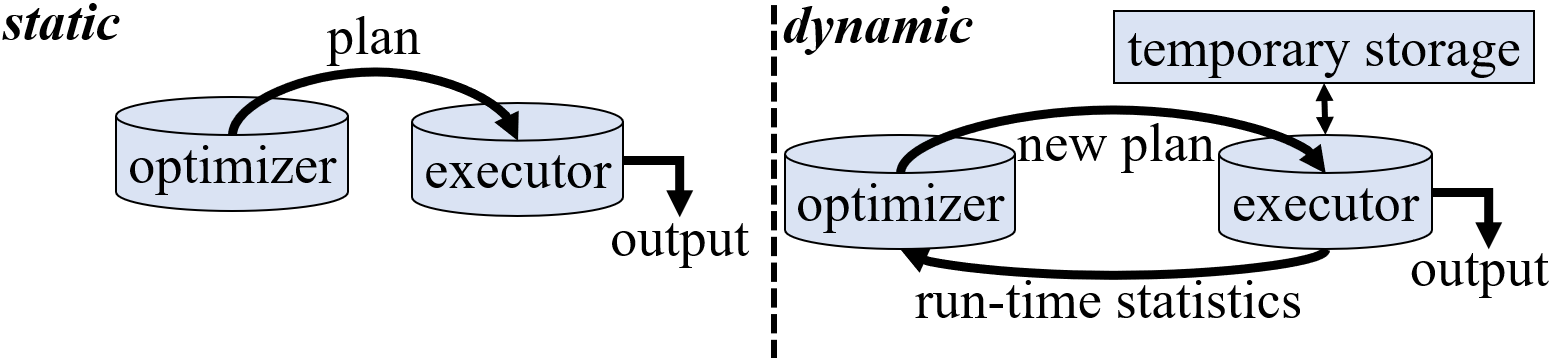
\includegraphics[width=\linewidth]{./pic/Figure1.png}
        \caption{Static and dynamic query optimization}
        \label{F1}
        \Description{In tradition structure, there is a unidirectional pipeline from optimizer to executor; and in breakup pipeline structure, there is a circle instead.}
    \end{figure}\par
    Re-optimization does not make drastic changes to the query execution engine. Instead, it detects during run-time whether the actual behavior of a query plan becomes significantly different from what was expected and attempts to correct the execution plan whenever it happens. In other words, re-optimization admits that the query optimizer can make mistakes in decisions and thus tries to alleviate them. In recent work, Perron et al. \cite{MichaelStonebraker} evaluated the performance of re-optimization on the Join Order Benchmark \cite{JOB}, and their result suggests that re-optimization can significantly reduce query execution time.\par
    Re-optimization makes use of the statistic of intermediate results, and in this paper, we refer to them as run-time statistics to distinguish them from statically collected statistics. By using run-time statistics, the optimizer improves cardinality estimation in two aspects: first, by replacing estimated statistics with run-time statistics, the optimizer reduces the cardinality estimation error caused by problematic assumptions. For example, the run-time statistics can include the actual distribution of attributes in the intermediate result, which leads to a more accurate cardinality estimation. Another aspect is that run-time statistics stop error propagation. The optimizer uses run-time statistics to replace the estimated cardinality, which essentially reduces the size of the join that needs to be estimated.\par
    Re-optimization can be classified as a specific case of the more general concept of adaptive query processing \cite{paper47}, in which query execution strategy changes adaptively based on the actual state during execution. Most existing adaptive query processing techniques keep the strict order between optimizer and executor. For example, parametric query optimization \cite{paper44} and Rio \cite{paper25} give the executor a set of possible optimal plans instead of giving one single plan. Thus, they can switch the plan during execution. Eddies \cite{paper30} generate a basic join tree by a simple pre-optimizer and can dynamically change the tuple pipeline in join operators during execution.

\subsection{Sub-plan Perspective} \label{S23}
\textcolor{blue}{
    We can summarize the general procedure of traditional re-optimization as follows:
    \begin{itemize}[leftmargin = 15pt]
        \item First, select a sub-tree of the global plan tree.
        \item Then, execute that sub-plan and materialize the result as a temporary table.
        \item Finally, replace the sub-tree with the table and re-optimize the remaining query.
    \end{itemize}
}\par
\textcolor{blue}{
    In traditional re-optimization, the materialized results are always the sub-trees of the global plan tree or so-called sub-plan. For example, in mid-query re-optimization \cite{Reopt}, the node whose subsequent operator is blocked (e.g., sort and hash) will be materialized. And in \textit{Pop} \cite{Pop}, the database system also materializes the sub-plans at the outer side of the nest-loop join. However, this sub-plan perspective has two problems.
}\par
\textcolor{blue}{
    First, re-optimization may be misled by the global plan if it deviates largely from the optimal one. Sub-plan perspective may choose a sub-plan that is the sub-tree of the global plan, but not the sub-tree of the optimal one. In that case, even if we re-optimize the remaining plan after executing the sub-plan, the join order still becomes sub-optimal. More seriously, as the problem scale of the remaining query is still large, the re-optimized plan can deviate significantly from the optimal plan again.
}\par
\textcolor{blue}{
    To illustrate how a bad global plan ruins re-optimization, we give the following example.
    \begin{Example}
        As shown in Figure \ref{F21}(a), due to an underestimation of cardinality, the global plan first decides to join relation $k$ and $mk$ by nest-loop join. However, in Figure \ref{F21}(b), the optimal choice is to join relation $ci$ and $n$ and then use the join result as a probe to index scan $k$ and $mk$. We assume a re-optimization happens immediately after the first join. Hence, the first sub-plan is $k \bowtie mk$, and we denote the materialized result as $S_1$. However, we still miss the opportunity to execute this query with the optimal execution plan. As shown in Figure \ref{F21}(c), the only way to correct back to the optimal plan is first to join $ci$ and $n$ in the re-optimized plan, but we cannot index scan $S_1$ as there is no index on the temporary relation. Instead, we have to use a hash join, which takes ten times more than index scan $k$ and $mk$.
    \end{Example}
}\par
    \begin{figure}[htb]
        \subfigure[\normalsize{Global plan}]
        {
            \begin{minipage}[t]{0.3\linewidth}
                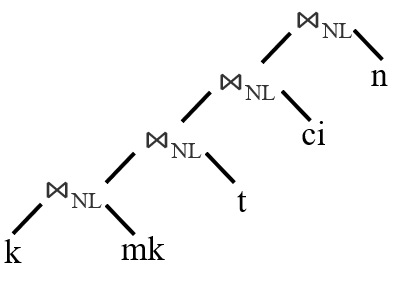
\includegraphics[width=\linewidth]{./pic/Figure21a.png}   
            \end{minipage}
        }
        \subfigure[\normalsize{Optimal plan}]
        {
            \begin{minipage}[t]{0.3\linewidth}
                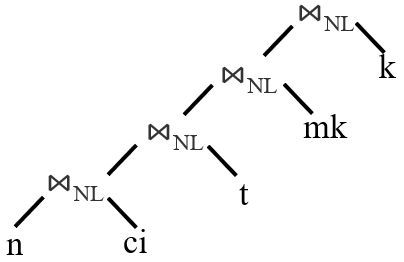
\includegraphics[width=\linewidth]{./pic/Figure21b.png}
            \end{minipage}
        }
        \subfigure[\normalsize{Re-Optimized plan after the first join}]
        {
            \begin{minipage}[t]{0.3\linewidth}
                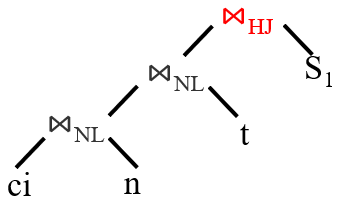
\includegraphics[width=\linewidth]{./pic/Figure21c.png}
            \end{minipage}
        }
        \centering
        \caption{Bad sub-plan example}
        \label{F21}
        \Description{}
    \end{figure}\par
\textcolor{blue}{
    And according to our observation, the phenomenon that the global plan hugely differs from the optimal one is not rare in the real world benchmark. Table \ref{T1} shows the ratio of queries whose global plans deviate hugely from the optimal plan in Join Order Benchmark. We will describe how to get the optimal plan in Section \ref{S5}. As shown in Figure \ref{F2}, we measure the similarity by the number of leaf nodes in the largest common sub-tree between the global plan and optimal plan: similarity is 0 means that the optimal plan is totally different from the global plan; 1 means they scan the same relation but do not join it with the same relation; and 2 means they execute the same first join, but their second joins are different.
}
    \begin{figure}[htb]
        \subfigure[\normalsize{Similarity is 0}]
        {
            \begin{minipage}[t]{0.3\linewidth}
                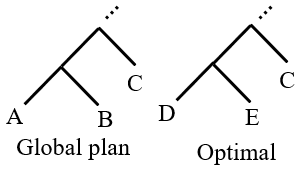
\includegraphics[width=\linewidth]{./pic/Figure2a.png}   
            \end{minipage}
        }
        \subfigure[\normalsize{Similarity is 1}]
        {
            \begin{minipage}[t]{0.3\linewidth}
                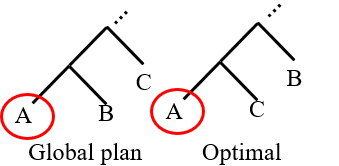
\includegraphics[width=\linewidth]{./pic/Figure2b.png}
            \end{minipage}
        }
        \subfigure[\normalsize{Similarity is 2}]
        {
            \begin{minipage}[t]{0.3\linewidth}
                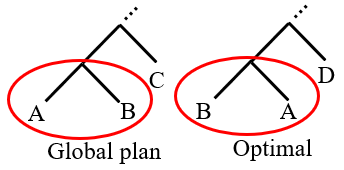
\includegraphics[width=\linewidth]{./pic/Figure2c.png}
            \end{minipage}
        }
        \centering
        \caption{The example of different similarity}
        \label{F2}
        \Description{}
    \end{figure}\par
\textcolor{blue}{
    From Table \ref{T1}, we can see that 13\% of the query plans completely deviate from the optimal plan, 12\% deviate from the optimal plan before the first join, and 32\% deviate from the optimal plan after the first join. In other words, no matter the size of the first sub-plan in sub-plan perspective, for 25\% queries in JOB, re-optimization will select the sub-optimal sub-plan at the beginning (similarity is 0 and 1). And suppose the first sub-plan has more than one join. In that case, re-optimization will choose a sub-optimal execution path for more than half queries (similarity is 0, 1 and 2).
}
    \begin{table}[htb]
        \caption{The ratio of queries whose global plans deviate hugely from the optimal plan}
        \label{T1}
        \begin{tabular}{c|c}
            \toprule
            Similarity & Ratio    \\
            \midrule
            0          & 13\%     \\
            1          & 12\%     \\
            2          & 32\%     \\
            > 2        & 43\%     \\
            \bottomrule
        \end{tabular}
    \end{table}\par
\textcolor{blue}{
    Second, for a given query, how often materialization will happen is unknown, which may incur a heavy overhead for materialization. In traditional re-optimizations, as we mentioned before, whether materialization happens depends on the type of plan nodes. We do not know whether and where the materialization will occur until the new plan becomes available. We call such a pattern the reactive pattern. The uncontrollability of materialization means non-robustness of the materialization overhead.
}\par
    
\subsection{Sub-query Perspective and Query Split Framework} \label{S24}
\textcolor{blue}{
    As the sub-plan perspective has the above problems, we propose a new perspective and reserve the general idea of changing the plan halfway through execution.
}\par
\textcolor{blue}{
    Different from materializing a sub-tree of the global plan (sub-plan), we split the query into sub-queries in advance and send them to the query processing engine as separate queries. Obviously, the global plan is discarded in this new perspective, and we call this perspective the \textit{sub-query perspective}.
}\par
\textcolor{blue}{
    Compared to the sub-plan perspective, our sub-query perspective has the following benefits:
    \begin{itemize}[leftmargin = 15pt]
        \item Do query optimization for each sub-query avoids the possible misleading of the global plan. Suppose a proper sub-query splitting strategy exists and a way to decide their execution orders (we will discuss them in Section \ref{S4}). In that case, the plan we get is more similar to the sub-tree of the optimal plan.
        \item As the size of each sub-query is small, according to Section \ref{S21}, the difficulty of query optimization decreases, and we can have more reliable execution plans for each sub-query.
        \item Because we split the query into sub-queries as soon as the query comes, we know exactly how often materialization will happen. Compared to the sub-plan perspective, our sub-query perspective is a proactive method. Thus, we ensure the robustness of the materialization overhead.
    \end{itemize}
}\par
    In this paper, we propose a new framework called \textit{query split} to cooperate with our sub-query perspective. In \textit{query split}, we execute a small part of the query each time and materialize its result until the entire query has been executed. Here we provide an example to demonstrate how \textit{query split} works in practice.
    \begin{Example}
        As shown in Figure \ref{F3}(a), we consider a query $G=R_1 \bowtie R_2 \bowtie R_3 \bowtie R_4 \bowtie R_5$ on five relations. First, we split query $G$ into three sub-queries, as shown in Figure \ref{F3}(b): $S_1=R_2 \bowtie R_3$, $S_2=R_3 \bowtie R_4 \bowtie R_5$, and $S_3=R_1 \bowtie R_2$. Then, we execute $S_1$ and materialize the result as temporary table $t_1$. Next, we replace $R_2$ and $R_3$ in $S_2$, $S_3$ by $t_1$, resulting in $S_2=t_1 \bowtie R_4 \bowtie R_5$, and $S_3=R_1 \bowtie t_1$, as shown in Figure \ref{F3}(c). Afterwards we execute the modified version of $S_2$, and materialize its result as $t_2$. Finally, as shown in Figure \ref{F3}(d), we replace $t_1$ in $S_3$ by $t_2$ to get $S_3=R_1 \bowtie t_2$, and then replan and execute it to obtain the result.
    \end{Example}
    \begin{figure}[htb]
        \subfigure[\normalsize{Join Graph of $G$}]
        {
            \begin{minipage}[t]{0.47\linewidth}
                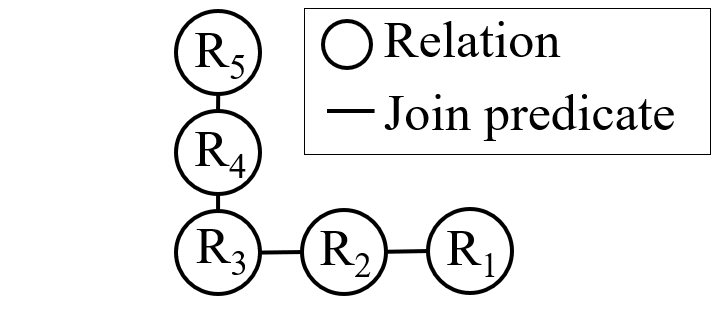
\includegraphics[width=\linewidth]{./pic/Figure3a.png}   
            \end{minipage}
        }
        \subfigure[\normalsize{$G$ with sub-queries $S_1$, $S_2$, $S_3$}]
        {
            \begin{minipage}[t]{0.47\linewidth}
                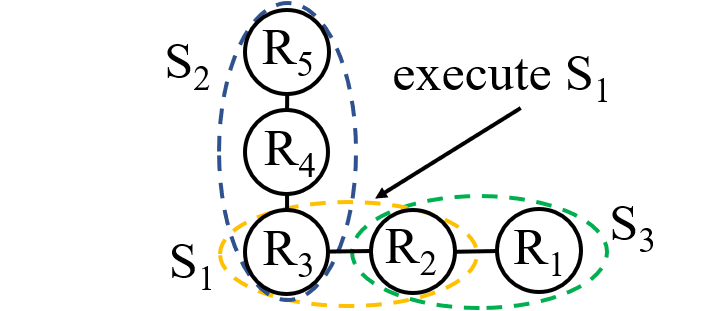
\includegraphics[width=\linewidth]{./pic/Figure3b.png}
            \end{minipage}
        }
        \subfigure[\normalsize{$G$ after executing $S_1$}]
        {
            \begin{minipage}[t]{0.47\linewidth}
                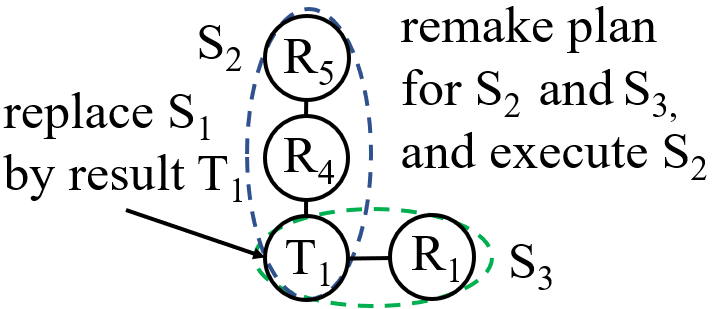
\includegraphics[width=\linewidth]{./pic/Figure3c.png}
            \end{minipage}
        }
        \subfigure[\normalsize{$G$ after executing $S_1$ and $S_2$}]
        {
            \begin{minipage}[t]{0.47\linewidth}
                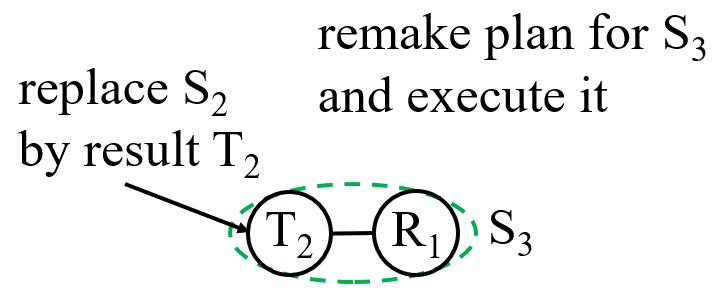
\includegraphics[width=\linewidth]{./pic/Figure3d.png}
            \end{minipage}
        }
        \centering
        \caption{\textit{query split} example}
        \label{F3}
        \Description{}
    \end{figure}\par
    More generally, \textit{query split} works as follows. First, for a given query, we split it into several small sub-queries by a sub-query splitting procedure. Then we compute the result of the original query using these sub-queries:
    \begin{itemize}[leftmargin = 15pt]
        \item Each time, choose a sub-query to execute and then remove it from the set of sub-queries.
        \item After running a sub-query $q_i$ and collecting run-time statistics, modify other sub-queries and remake their execution plans.
        \item When no sub-query is left, merge some sub-queries results to obtain the original query result.
    \end{itemize}\par
\textcolor{blue}{
    \textit{Query split} framework has two characteristics:
    \begin{itemize}[leftmargin = 15pt]
        \item Traditional re-optimization techniques determine the sub-query (sub-plan) to be executed after query optimization. In contrast, query split determines what sub-queries will be executed before the query optimization stage.
        \item \textit{Query split} can also implement the re-optimization with the sub-plan perspective by designing a specific splitting algorithm. We use the global plan as an input for the query splitting algorithm, and every time a sub-query is executed, we do query splitting again.
    \end{itemize}
}\par
    \textit{Query split} is a new attempt at re-optimization, and we hope to use this work to draw more attention and research to this direction. Our new framework opens a fresh perspective to the query optimization problem. As shown in Section \ref{S5}, \textit{query split} outperforms the built-in PostgreSQL optimizer by a large margin and reaches near-optimal execution time in the Join Order Benchmark.